\documentclass[a4paper, 12pt]{article}

\usepackage{amsthm, amsfonts,amssymb,epsfig,amsmath,minted,graphicx,hyperref}
\usepackage[margin=0.5in]{geometry}

\setlength\parindent{0pt}

\title{\textbf{CMPE 121 Lab Project} \\ 
    \textbf{Othello (Reversi) for the PSoC-5 Microcontroller}}
\author{Amlesh Sivanantham \\ (asivanan) \\ 1388793}
\date{December 6, 2016}

\begin{document}
	
	\maketitle

	\section{Introduction} 

	The purpose of this lab project was to implement a fully functioning
    game called Othello (Reversi) on the PSoC-5 Microcontroller which built
    on everything we have learned up to this point in the class. The goals at
    the end of the final project were that we would have learned to create
    a functioning hardware and software component. I will go over the whole
    process and go over core functionality of the project in the order that I
    implemented it. However, I will start by explaining the process of
    setting up the hardware first, but it should be noted that each hardware
    component was built only when it came time to implement it in software.
    There are many features that I wanted to implement as well, but do to time
    constraints I was unable to start them. I will ultimately finish
    the features I didn't implement over the winter break. I will go over the
    details of what those features are in the Conclusion section.

    \section{Hardware Design}
 
    There were three components that were required to be connected to the
    microcontroller for this project. They were the RGB LED Matrix, Wifi
    Controller, and the SD Card Reader. As mentioned before, each part was
    only implemented when it came to implement it's respective software
    component. However, It should be noted that first, the breadboard
    was used to prototype the component and test it with the code. Once that
    was verified, it was verified that it was working correctly, the
    components were soldered onto the Perf Board provided to us in the Lab
    Kits. All initial schematics were drawn by hand. 
    \\ \\
    This class was the first time I was introduced to soldering, so I was
    bound to make a mistake. In the process of soldering I made bad
    connections and burnt myself once. This was alright however since I was
    able to verify the my circuit with continuity checks. I had to get a
    replacement SD Card Reader however. In the process of soldering, I
    initially placed the pins the wrong way. Removing the pins was literally
    impossible, but eventually I was able to remove the pins. However there
    was still some leftover solder covering the holes where the pins should
    go. Hence I needed to use the soldering iron and the solder remover to
    remove that remaining solder. Sadly, in the process of removing the
    solder, I managed to burn away the metal plate. Luckily BELS was kind
    enough to allow me to get it replaced for free (it is \$10 normally).
    
    \clearpage
    Seen below are pictures of the schematic and actual perf board after
    soldering was finished.

    \begin{figure}[H]
        \centering
        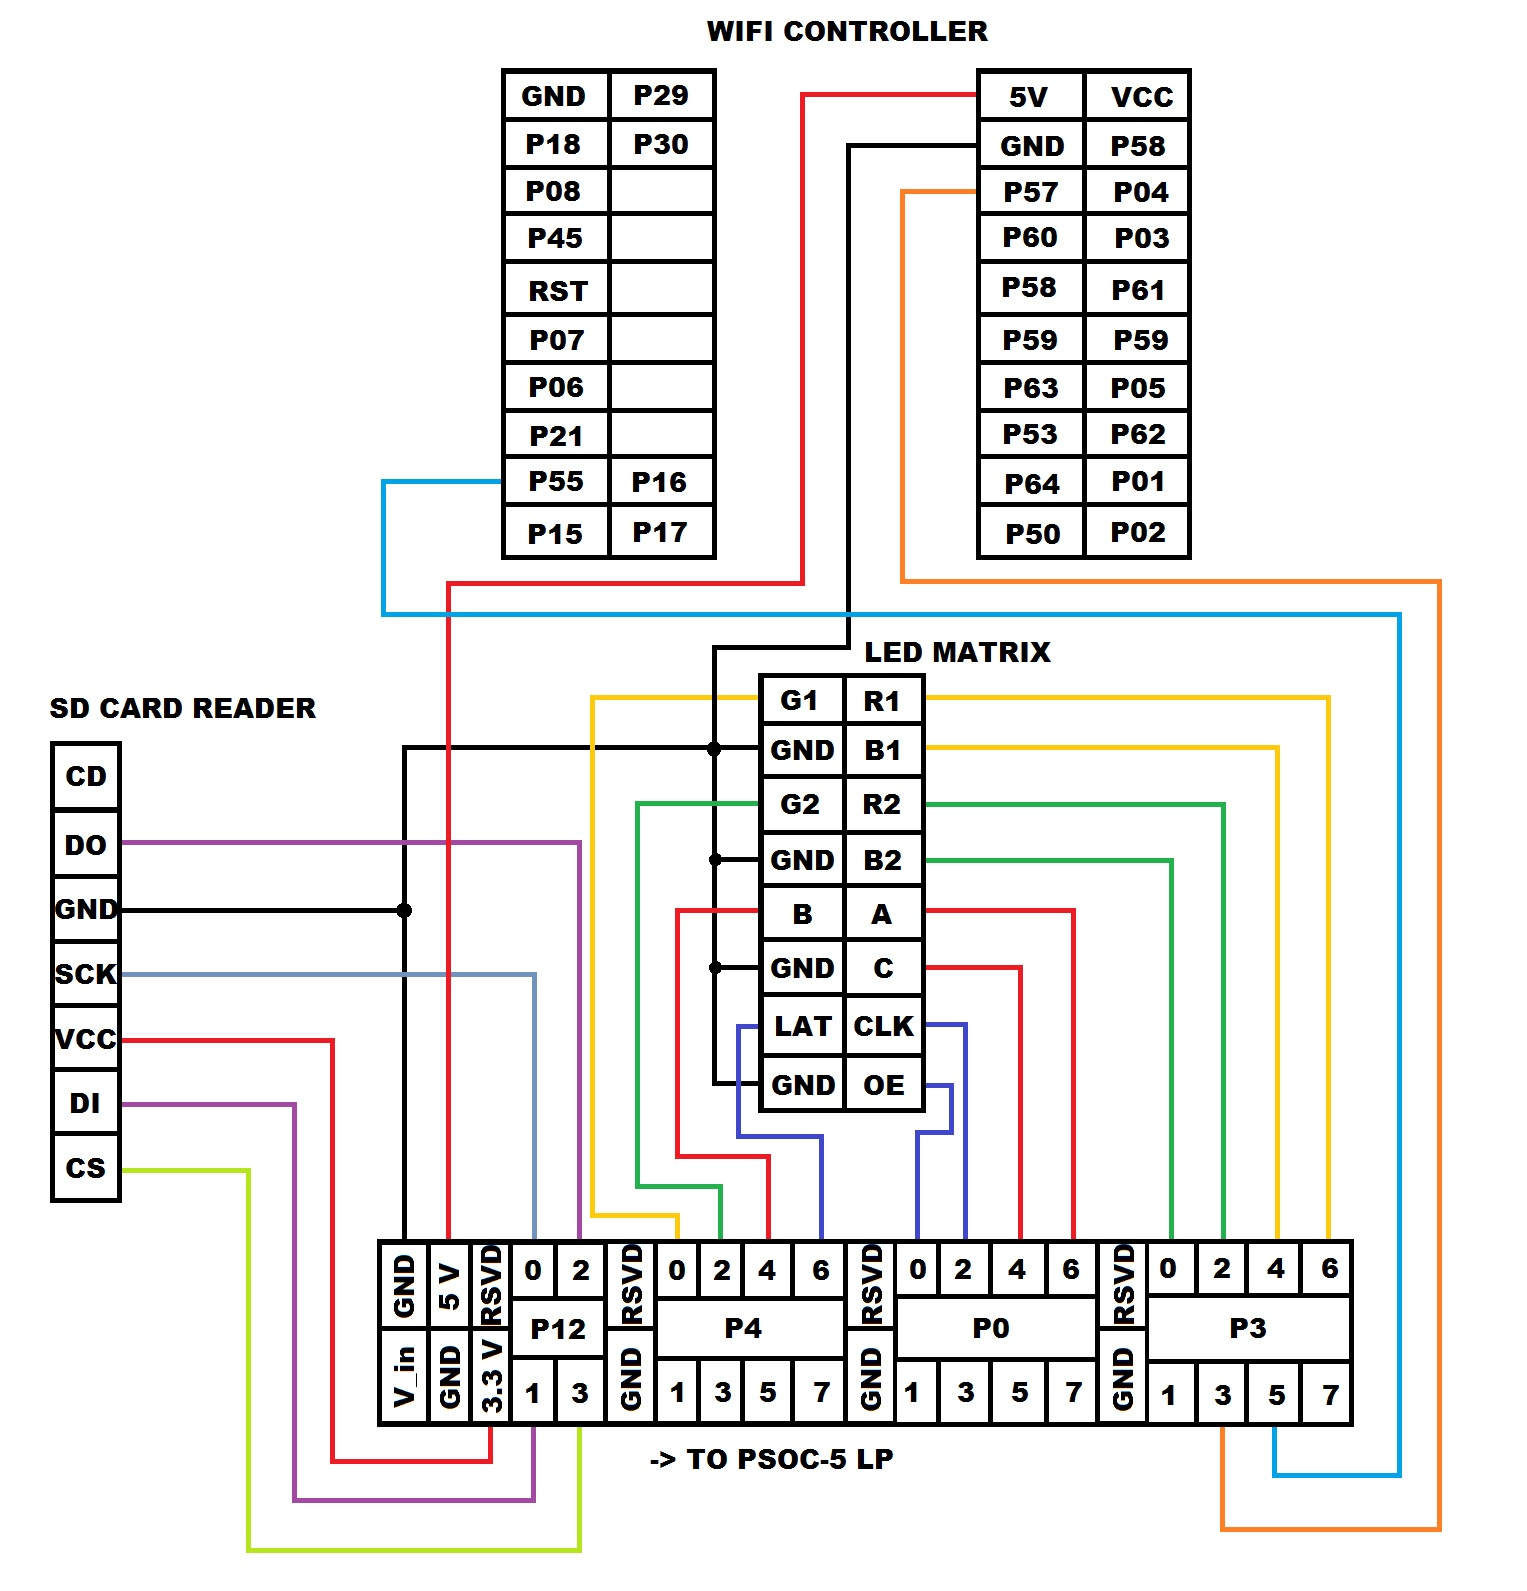
\includegraphics[scale=0.3]{pics/perf}
        \caption{A rough schematic of the connections found on the Perf Board}
        \label{fig:SolderSetup}
    \end{figure}

    \begin{figure}[H]
        \centering
        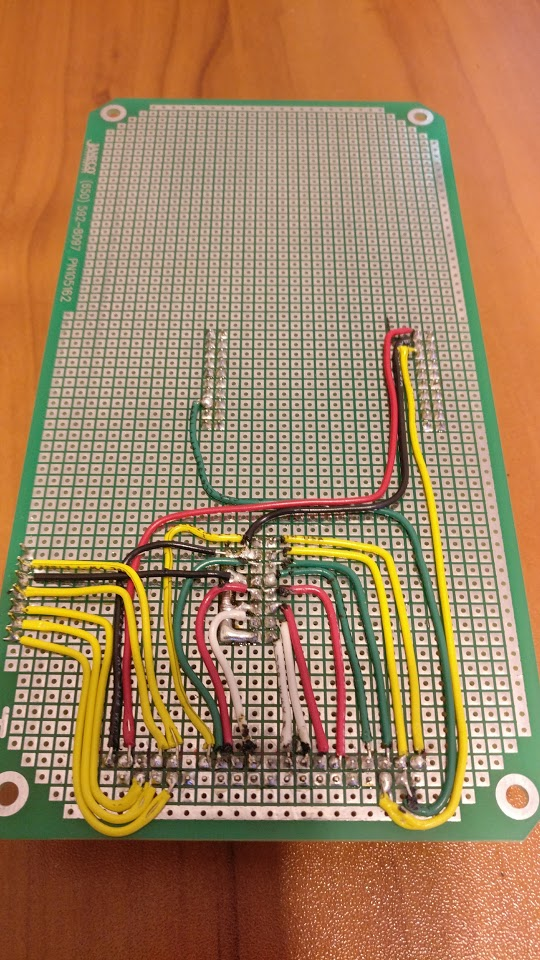
\includegraphics[scale=0.3]{pics/perfBoard}
        \caption{A look at the actual Perf Board}
        \label{fig:PerfSetup}
    \end{figure}

    \section{Software Design}

    \subsection{Workflow and Overview}

    For this lab, I initially made a flowchart of how I wanted to proceed.
    Originally, I made the flowchart on paper, but for the sake of
    convenience, I have made it digital. You can see it below. For each
    section I have made a list of high level goals that I wished to
    implement. Unfortunately, I was not able to get to all of them. 

    \begin{figure}[H]
        \centering
        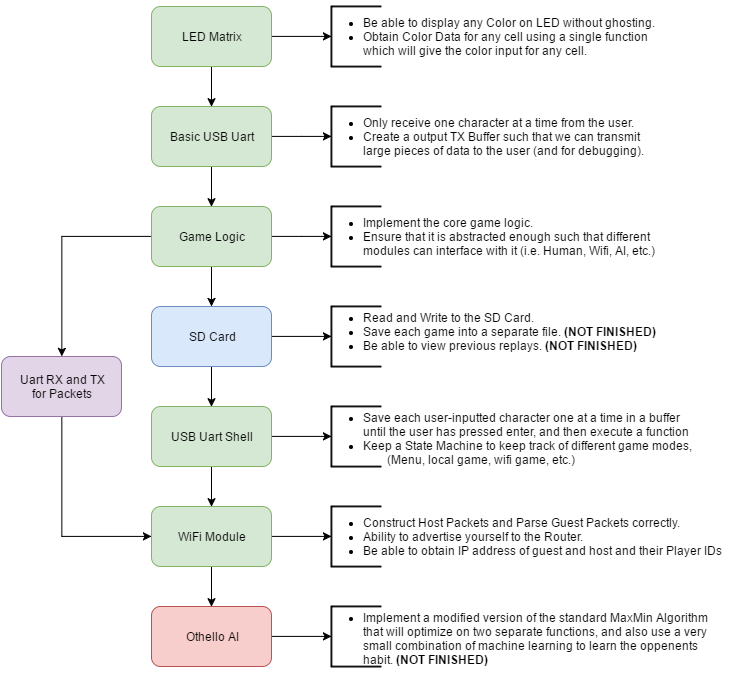
\includegraphics[scale=0.7]{pics/othelloFlow}
        \caption{A look at the actual Perf Board}
        \label{fig:PerfSetup}
    \end{figure}

    Essentially I setup a header file for each module to keep things
    abstracted. In the next few sections I will go over these modules and
    their functionality and constraints, but before we proceed, we will need
    to understand what the file \textit{main.c} does.

\end{document}
